\documentclass[pstricks,border=14pt,14pt]{article}
\usepackage{pst-plot}
\usepackage[a4paper, margin=1in]{geometry}
\usepackage[english]{babel}
\usepackage[utf8]{inputenc}
\usepackage{biblatex}
\usepackage{listings}
\usepackage{graphicx}
\usepackage{sectsty}
\usepackage{float}
\usepackage{multirow}
\usepackage[T1]{fontenc}
\usepackage{fancyhdr}
% \usepackage[p,osf,swashQ]{cochineal}
% \usepackage{cabin}
% \usepackage[varqu,varl,scale=0.9]{zi4}

\sectionfont{\fontsize{12}{11.5}\selectfont}
\subsectionfont{\fontsize{11.5}{9.5}\selectfont}


\pagestyle{fancy}
\fancyhf{}
\rhead{TING-WEI SU}
\lhead{CSCE 735 700}
\title{Quick Sort on a Hypercube - Major Project}
\author{TING-WEI SU (UIN:231003210) & willytwsu@tamu.edu & CSCE-735}
\date{}

\addbibresource{reference.bib}
\begin{document}

\maketitle 
%------------------------------------------------------------------------------------------
%Part A
\part*{Part A: Developement}
\subsection*{1. (60 points) Complete the MPI-based code provided in qsort\_hypercube.cpp to implement the parallel quicksort algorithm for a d-dimensional hypercube with $p=2d$ processors. 40 points will be awarded if the code compiles and executes the following command successfully.}
The solution source code, the qsort\_hypercube.c file is attached.
\begin{verbatim}
mpirun -np 2 ./qsort_hypercube.exe 4 -1
mpirun -np 4 ./qsort_hypercube.exe 4 -2
mpirun -np 8 ./qsort_hypercube.exe 4 -1
mpirun -np 16 ./qsort_hypercube.exe 4 0
mpirun -np 16 ./qsort_hypercube.exe 20480000 0
\end{verbatim}
Output:
\begin{verbatim}
[willytwsu@grace2 Major_Project]$ mpirun -np 2 ./qsort_hypercube.exe 4 -1
[Proc: 0] number of processes = 2, initial local list size = 4, hypercube quicksort 
time = 0.003159
[Proc: 0] Congratulations. The list has been sorted correctly.
[willytwsu@grace2 Major_Project]$ mpirun -np 4 ./qsort_hypercube.exe 4 -2
[Proc: 0] number of processes = 4, initial local list size = 4, hypercube quicksort 
time = 0.001971
[Proc: 0] Congratulations. The list has been sorted correctly.
[willytwsu@grace2 Major_Project]$ mpirun -np 8 ./qsort_hypercube.exe 4 -1
[Proc: 0] number of processes = 8, initial local list size = 4, hypercube quicksort 
time = 0.005848
[Proc: 0] Congratulations. The list has been sorted correctly.
[willytwsu@grace2 Major_Project]$ mpirun -np 16 ./qsort_hypercube.exe 4 0
[Proc: 0] number of processes = 16, initial local list size = 4, hypercube quicksort 
time = 0.010782
[Proc: 0] Congratulations. The list has been sorted correctly.
[willytwsu@grace2 Major_Project]$ mpirun -np 16 ./qsort_hypercube.exe 20480000 0
[Proc: 0] number of processes = 16, initial local list size = 20480000, hypercube quick
-sort time = 2.712228
[Proc: 0] Congratulations. The list has been sorted correctly.
\end{verbatim} 
%end of Part A
%------------------------------------------------------------------------------------------
%Part B
\part*{Part B: Scalability Study}
\section*{{Weak Scalability Study}
\subsection*{3. (5 points) In your own words, describe what is meant by weak scalability, i.e., what does it mean that an algorithm or implementation is “weakly” scalable. If you use a textbooks or an online resource as reference, then include a citation.}
Weak scalability is not like the literal meaning saying that the scalability is negative or what. It simply state that the problem size of the parallel computing structure will increase along with the process number. When the node of the computing power increase, the problem size will increase as well.}
\subsection*{4. (15 points) Run your code to sort a distributed list of size $n \times p$ where n is the size of the local list on each process and p is the number of processes. For your experiments, use n=20,480,000 and p = 1, 2, 4, 8, 16, 32, and 64. Set type=0. Plot the execution time, speedup, and efficiency of your code as a function of p. Use logarithmic scale for the x-axis. \\ Note that the size of the list to be sorted is proportional to the number of processes p. In order to get speedup for a specific value of p, you need to determine the execution time to sort a list of size $n \times p$ with one process. As an example, speedup for $p = 4$ is the ratio of execution time for a list of size 81,920,000 with one process (T1) to the execution time for a list of size 20,480,000 with 4 processes (T4).}
\section*{Strong Scalability Study}
\begin{figure}[H]
    \centering
    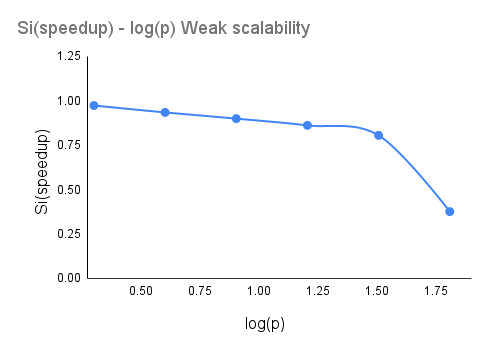
\includegraphics[width=12cm]{Weak_scalability_Si_logP.png}
    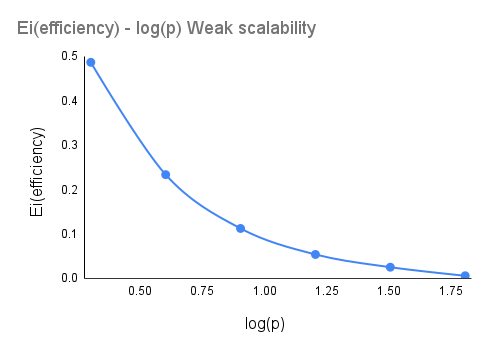
\includegraphics[width=12cm]{Weak_scalability_Ei_logP.png}
    \caption{k = 20}
    \label{fig:my_label}
\end{figure}
\subsection*{5. (5 points) In your own words, describe what is meant by strong scalability, i.e., what does it mean that an algorithm or implementation is “strongly” scalable. If you use a textbooks or an online resource as reference, then Include citations as appropriate.}
Strong scalability stated that the problem size will remain the same as the number of the process increase whatsoever. 

\subsection*{6. (15 points) Now run your code with n=20,480,000/p where p = 1, 2, 4, 8, 16, 32, and 64. Set type=0. Plot the execution time, speedup, and efficiency of your code as a function of p. Use logarithmic scale for the x-axis.
Unlike the weak scalability study, here the size of the list to be sorted remains unchanged at 20,480,000 even as you increase the number of processes. To determine speedup for any p you need to compare the execution time on p processes to the execution time for a list of size 20,480,000 with one process.}
%Part B.Graph
\begin{figure}[H]
    \centering
    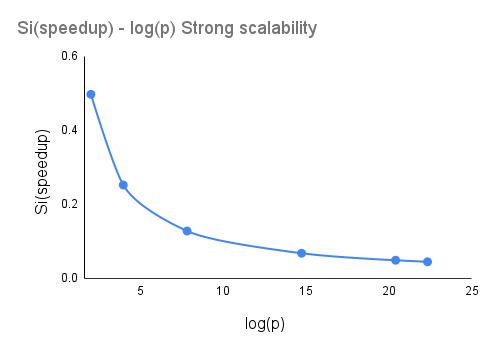
\includegraphics[width=12cm]{Strong_scalability_Si_logP.png}
    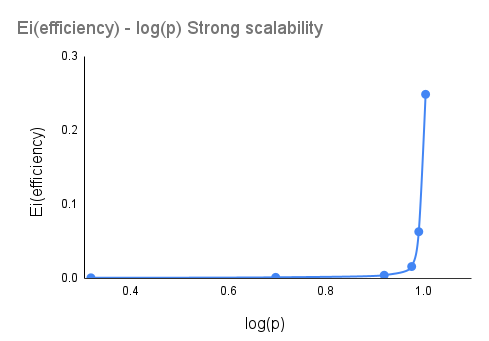
\includegraphics[width=12cm]{Strong_scalability_Ei_logP.png}
    \caption{k = 28}
    \label{fig:my_label}
\end{figure}
%------------------------------------------------------------------------------------------
%Part B.Comments
%end of Part B
%------------------------------------------------------------------------------------------
\newpage
\subsection*{Reference}
$[1]$ \url{https://hpc-wiki.info/hpc/Scaling_tutorial#Strong_or_Weak_Scaling} \\
$[2]$ \url{https://www.kth.se/blogs/pdc/2018/11/scalability-strong-and-weak-scaling} \\
$[3]$ Amdahl, G.M. Validity of the single-processor approach to achieving large scale computing capabilities.In AFIPS Conference Proceedings vol. 30 (Atlantic City, N.J., Apr. 18-20). AFIPS Press, Reston, Va.,1967, pp. 483-485 \\
$[4]$ REEVALUATING AMDAHL'S LAWJOHN L. GUSTAFSON \\
%\printbibliography %Prints bibliography
\end{document}
